\documentclass[letterpaper]{article} \usepackage[submission]{aaai2027}  \usepackage[hyphens]{url}  \usepackage{graphicx} \urlstyle{rm} \def\UrlFont{\rm}  \usepackage{natbib}  \usepackage{caption} \frenchspacing  

\usepackage{booktabs}
\usepackage{amsmath}
\usepackage{array}

\pdfinfo{
/TemplateVersion (2027.1)
}

\setcounter{secnumdepth}{1}
\newcommand{\TODO}[1]{\textcolor{red}{\textbf{TODO:}~#1}}

\title{Looking Is Not Grounding: A Diagnostic Framework for Attention-Based Hallucination Detection and Mitigation in LVLMs}

\author{Anonymous Submission}
\affiliations{}

\begin{document}
\maketitle

\begin{abstract}
Attention is widely used as a proxy for visual grounding in large vision--language models (LVLMs): detectors score how object tokens attend to the image, while mitigation methods amplify or redistribute visual attention to reduce hallucinations. We argue that this premise is incomplete: visual attention allocation is not object-level evidence verification. Attention can be plausibly but incorrectly grounded, routing to regions semantically associated with the target object without verifying the target itself. We propose a verification-centered diagnostic framework for testing this proxy in both detection and mitigation. On the detection side, we show that strong attention-based AUROC can be driven by \emph{generation-position confounding}. On LLaVA-1.5-7B over MSCOCO ($16{,}426$ object mentions), position alone reaches $0.830$ AUROC; under within-bin, matched-pair, same-object, and residual evaluation, attention-mass detectors such as PAS and SVAR retain only a small fraction of their above-chance signal, while representation and uncertainty baselines remain more robust. A purpose-built attention-shape stress test, SinkDetect, also collapses under position control. On the mitigation side, we reproduce attention-intervention components of PAI, ClearSight, and Visual Attention Sink on POPE and CHAIR. ClearSight mainly shifts POPE answers toward ``yes'' (TPR $+3.5$ points, FPR $+3.8$ points), while an attention-shift audit shows that PAI increases active-layer visual attention by $+0.038$ without changing any adversarial POPE decisions. These results suggest that attention can contain grounding information, but simple attention scores and attention amplification do not by themselves verify whether a visual claim is supported.
\end{abstract}
 \section{Introduction}

Large vision--language models (LVLMs) such as LLaVA-1.5 \cite{liu2023llava} produce fluent image descriptions, but they often \emph{hallucinate}: they mention objects that are not present in the image. Because hallucination is a grounding failure, a natural response has been to inspect or manipulate the model's visual attention. Detection methods score how much, or where, an object token attends over the image \cite{jiang2024devils,hoangxuan2026pas}; mitigation methods amplify image attention or redistribute attention away from sinks \cite{liu2024pai,yin2025clearsight,kang2025visualsink}. These approaches share an appealing premise: better visual attention should imply better visual grounding.

This paper studies a gap in that premise through a verification-centered diagnostic framework: \textbf{attention allocation is not evidence verification}. Attention tells us where computation is routed, but object hallucination depends on whether a specific object claim is supported by visual evidence. The distinction matters in two directions. A detector can assign high hallucination scores because attention statistics correlate with a nuisance variable rather than grounding. A mitigation method can make the model look more at the image, yet still fail to distinguish whether the queried object is present or absent.

A central mechanism is what we call \emph{associated-evidence grounding}. An LVLM may attend to a real visual region that is related to the queried object, while the queried object itself is absent. For example, when asked whether an image contains a \emph{sink}, a model may route attention to a visible \emph{toilet} or bathroom context, activate co-occurrence and embedding-space associations, and answer ``yes.'' The attention map is not random: it points to meaningful visual evidence. But the evidence is not \emph{target-discriminative}. This mechanism is consistent with analyses that connect object hallucination to overconfidence in irrelevant visual features after visual tokens are projected into the language embedding space \cite{bai2025adavib}. It clarifies why attention-based methods can fail even when the model is genuinely looking at the image.
\TODO{Add a compact mechanism figure contrasting target-discriminative evidence with associated evidence, e.g., sink query / toilet region / false yes.}

We first expose this problem on the detection side through \textbf{generation-position confounding}. Captions are produced autoregressively, and the position of an object token affects both the feature and the label. As decoding proceeds, attention shifts from image tokens toward generated text; at the same time, hallucinations become more frequent late in the caption. On our LLaVA-1.5-7B / MSCOCO run, the hallucination rate rises from $2.2\%$ in the first ten generated tokens to over $60\%$ past position 100. A score that tracks position can therefore appear to detect hallucination without testing visual support.

This confound is strong enough to reorder the field's apparent progress. A trivial detector using only generation position reaches $0.830$ AUROC, comparable to or higher than attention baselines. Under our position-controlled protocol---within-bin, matched-pair, and residual AUROC---PAS and SVAR drop from $\sim$$0.83$ overall AUROC to $\sim$$0.58$ within-bin AUROC, retaining only $22$--$28\%$ of their above-chance signal. Representation and uncertainty baselines such as Internal Confidence (IC), entropy, and NLL retain substantially more signal. Even SinkDetect, our stress-test detector built to use purified visual-attention shape rather than mass, collapses to chance under position control.

We then ask whether the same proxy failure appears in \emph{attention-based mitigation}. If visual attention were a reliable grounding handle, amplifying or re-routing it should improve hallucination behavior, not merely change output tendencies. We reproduce the attention-intervention components of PAI, ClearSight, and Visual Attention Sink on POPE and CHAIR. The results are cautionary: PAI-attention-only gives essentially no benefit; ClearSight increases POPE recall but also increases false positives by a comparable or larger amount; and Visual Attention Sink makes captions longer, mentions more objects, and hallucinates more object mentions. These failures are consistent with the same mechanism: increasing visual influence can amplify associated evidence, visual plausibility, or object richness without improving object-presence verification.

Studying detection and mitigation together is important because the two literatures often validate the same proxy in opposite directions. A detector treats an attention pattern as a measurement of grounding; an intervention treats a modified attention pattern as a mechanism for improving grounding. If the proxy is valid, the same signal should remain selective under nuisance controls and should improve object-presence discrimination when amplified. If it is invalid, both tasks can show attractive aggregate gains for the wrong reason. This paper uses that symmetry as a diagnostic tool: detection experiments reveal whether attention scores measure object evidence, mitigation experiments reveal whether attention changes cause object verification, and associated-evidence audits test whether plausible visual evidence is actually target-discriminative.

\paragraph{Contributions.} We make six contributions.
\begin{itemize}
\item We identify generation-position confounding in token-level LVLM hallucination detection and show that position alone reaches $0.830$ AUROC on LLaVA-1.5-7B / MSCOCO (\S\ref{sec:protocol}).
\item We introduce a verification-centered diagnostic framework and instantiate it with position-controlled detection metrics, answer-prior mitigation metrics, attention-shift selectivity audits, and semantic-neighbor negative slices (\S\ref{sec:protocol},~\S\ref{sec:associated-audit}).
\item We re-evaluate detection baselines spanning uncertainty, representation, and attention signals (\S\ref{sec:protocol},~\S\ref{sec:results}).
\item We build SinkDetect as a stress test of carefully engineered attention-shape features and show that even purified attention shape does not yield position-independent detection signal in this setting (\S\ref{sec:sinkdetect}).
\item We extend the critique to attention-based mitigation by evaluating PAI-attention-only, ClearSight, and Visual Attention Sink under POPE yes-prior diagnostics and CHAIR caption statistics (\S\ref{sec:mitigation}). The results support our central claim: looking is not verifying.
\item We identify associated-evidence grounding as a mechanism that links the detection and mitigation failures: attention can select visually meaningful but non-discriminative evidence, so future methods must test target-object verification rather than visual routing alone.
\end{itemize}
 \section{Related Work}
\label{sec:related}

\noindent\textbf{Object hallucination detection in LVLMs.}
Object hallucination was formalized as an image-captioning failure by CHAIR \cite{rohrbach2018chair} and has since become a central reliability problem for LVLMs. Recent detectors differ in what internal signal they treat as evidence. Uncertainty methods use the output distribution, such as token likelihood or entropy. Representation methods, such as IC, use internal visual representations to estimate whether the object is supported \cite{jiang2024interpreting}. Attention-based methods instead score how object tokens route computation: SVAR uses object-to-image attention mass \cite{jiang2024devils}, PAS measures attention to preliminary generated tokens \cite{hoangxuan2026pas}, and recent fine-grained grounding scores combine patch-level dispersion and consistency \cite{beyond2026global}. Our work is not another detector in this line. It asks whether these signals remain selective for object evidence after controlling for generation position and object identity.

\noindent\textbf{Attention-based hallucination mitigation.}
Training-free mitigation methods often intervene during decoding by changing either logits or attention. VCD-style methods contrast visual and language-biased predictions, while PAI increases visual attention and combines the attention branch with contrastive/CFG-style decoding in the full method \cite{liu2024pai}. ClearSight amplifies mid-layer image signals and suppresses prefix influence \cite{yin2025clearsight}. Visual Attention Sink redistributes mass away from high-activation sink tokens toward visual tokens \cite{kang2025visualsink}. These methods are motivated by the same intuition as attention detectors: stronger or cleaner visual routing should improve grounding. We evaluate the attention-intervention components under answer-prior and attention-selectivity controls, because a method can increase recall or object richness without improving object-presence verification.

\noindent\textbf{Evaluation shortcuts and evidence verification.}
Several recent analyses show that LVLM hallucination benchmarks can reward shortcut behavior. The Mirage study argues that contrastive-decoding gains on POPE can come from output-distribution shifts rather than genuine mitigation \cite{yin2025mirage}. AdaVIB connects hallucination to overconfidence in irrelevant visual features after visual tokens enter the language embedding space \cite{bai2025adavib}. These findings motivate a stricter question than whether the model attends to the image: does the attended evidence verify the target object claim? Our diagnostic protocol extends this question to both detection and mitigation by combining position control, answer-prior control, attention-shift selectivity, and semantic-neighbor negatives.
 \section{Attention as a Proxy}
\label{sec:proxy}

Attention-based hallucination methods share a convenient but under-tested proxy: they treat where an LVLM routes computation as evidence for whether an object claim is visually supported. Detection methods instantiate this proxy by converting attention into a scalar score. SVAR sums object-to-image attention mass \cite{jiang2024devils}; PAS measures object-token attention to previously generated prelim tokens \cite{hoangxuan2026pas}; and recent fine-grained detectors combine patch attention dispersion with cross-modal consistency \cite{beyond2026global}. These methods are attractive because they are training-free and internally available, but their scores still summarize routing rather than verification.

Mitigation methods instantiate the same proxy operationally. PAI increases image-token attention logits and combines this with contrastive/CFG decoding in the full method \cite{liu2024pai}; ClearSight scales mid-layer text-to-image attention and suppresses system-prefix attention \cite{yin2025clearsight}; Visual Attention Sink redistributes mass from high-activation sink tokens toward non-sink visual tokens \cite{kang2025visualsink}. All three are motivated by the idea that increasing useful visual attention should improve grounding. The recent ``Mirage'' analysis of contrastive decoding shows that POPE gains can instead come from output-distribution shifts and decoding constraints rather than hallucination mitigation \cite{yin2025mirage}. We ask whether attention-side methods suffer an analogous failure: their routing changes may be real, while their grounding gains are not.

\begin{table}[t]
\centering
\scriptsize
\setlength{\tabcolsep}{3.0pt}
\begin{tabular}{p{0.23\columnwidth}p{0.32\columnwidth}p{0.32\columnwidth}}
\toprule
Use & Proxy & Failure mode tested \\
\midrule
Detection & attention mass or shape is a grounding score & score tracks generation position or object frequency \\
Mitigation & more visual routing reduces hallucination & output prior or caption style shifts without verification \\
Stress test & purified shape removes mass bias & normalized shape still tracks decoding dynamics \\
\bottomrule
\end{tabular}
\caption{The shared proxy behind the methods we test. The paper evaluates whether the proxy survives controls that target its most likely failure mode.}
\label{tab:proxy}
\end{table}
 

The missing distinction is between \emph{allocation} and \emph{verification}. Allocation says that a token attends to the image, to prior text, or to a sink position. Verification asks whether the image contains the object being claimed. A method that only changes allocation can increase visual plausibility, object richness, or the probability of answering ``yes'' without checking object presence. This distinction motivates our diagnostic design: every score or intervention is evaluated not only by its aggregate metric, but also by whether it remains selective after controlling for nuisance variables and output-prior shifts.

\paragraph{Associated evidence is not target evidence.} The allocation--verification gap is sharpest when the attended region is meaningful but non-discriminative. In many hallucinations, the visual evidence is not arbitrary noise: it is a nearby object, a scene context, or a visual token whose language-space neighborhood is associated with the target. A bathroom region may support the prior that a sink is plausible, but it is not evidence that a sink is present. This is precisely the case where attention explanations are most tempting and most dangerous: the heatmap looks visually sensible, while the object-level claim is false. We therefore treat \emph{target-discriminative selectivity} as the missing criterion. A useful detector should separate present and absent instances of the same object under comparable position and context; a useful intervention should increase grounding for true positives more than for false positives.

This framing also explains why a negative result on simple attention scores is still informative. Attention may participate in the computation that supports grounding, but a scalar proxy must be stable to nuisance variables and selective for object evidence. If a score only becomes strong when late objects are more likely to hallucinate, or if an intervention increases visual routing for both true and false positives, then the method has not measured verification. Our experiments therefore focus less on whether attention changes and more on whether the change is \emph{selective} in the direction that grounding requires.
 \section{Diagnostic Protocol}
\label{sec:protocol}

Our detection protocol starts from a confound that aggregate AUROC hides. Let an object mention be generated at position $p$, and let $y$ indicate whether CHAIR marks it hallucinated. On LLaVA-1.5-7B / MSCOCO, the hallucination rate rises from $2.2\%$ in the first ten generated tokens to above $60\%$ after position 100. At the same time, many attention statistics drift with decoding position as the model moves from image-conditioned prefix processing toward generated text. Thus position acts as a common cause $p\rightarrow s$ and $p\rightarrow y$ for a detector score $s$: a score can obtain high AUROC by tracking where the object appears in the caption rather than whether the image supports it. The confound is large enough that position alone reaches $0.830$ AUROC.

This confound is not a small calibration nuisance. AUROC is a pairwise ranking metric: it asks whether a random hallucinated mention receives a higher score than a random grounded mention. If hallucinated mentions are late and grounded mentions are early, a position-tracking score will win many cross-position pairs while failing all same-position comparisons. This is why we do not treat overall AUROC as a sufficient hallucination-detection metric. It remains useful for comparability with prior work, but it cannot establish that a detector reads visual evidence.

We therefore report aggregate metrics only as a diagnostic baseline and use four position-controlled metrics as the main test. \textbf{Within-bin AUROC} computes AUROC inside generated-token bins of width 10 and averages valid bins by size. \textbf{Matched-pair AUROC} compares hallucinated mentions only against grounded mentions within $\pm5$ generated tokens. \textbf{Residual AUROC} removes $E[s\mid p]$ before scoring; we use fixed-bin residuals by default and also report linear, cubic, and quantile-bin variants. \textbf{Same-object matching} further restricts matched pairs to the same generated object word, addressing category-frequency confounds. A genuinely grounded detector should retain discrimination under these controls; a positional proxy should collapse toward chance.

Our mitigation protocol mirrors the same logic. Standard POPE accuracy or F1 can improve when a method shifts the yes/no answer prior, so we report yes rate, TPR, FPR, MCC, and $\Delta\mathrm{TPR}-\Delta\mathrm{FPR}$ rather than treating recall gains alone as mitigation. CHAIR captioning is evaluated with CHAIR$_i$, CHAIR$_s$, mean caption length, object mentions, and hallucinated-object mentions, because a method can lower hallucinations by producing shorter or less object-rich captions. Finally, we add an attention-shift audit on adversarial POPE: for each intervention we record pre/post visual, prefix, and sink attention mass in active layers and compare true positives against false positives. This audit tests whether the intended routing change is selective for verified object presence.

The associated-evidence audit adds a harder verification slice. Instead of asking only whether the target object is absent, it asks whether a method remains reliable when a related object or scene context is present. These semantic-neighbor negatives are the cases in which attention can look most persuasive while still failing the target-object claim. A detector should not mark them as grounded simply because the attention map is coherent; a mitigation method should not increase their yes rate simply because the image contains plausible associated evidence.

The protocol is intentionally diagnostic rather than leaderboard-oriented. It follows the spirit of the contrastive-decoding critique in \citet{yin2025mirage}: when a benchmark reward can be obtained by a simpler spurious mechanism, the evaluation must separate intended causal effect from shortcut behavior. For detection, the shortcut is generation position. For mitigation, the shortcut is answer-prior or caption-style movement. In both cases, the question is the same: does the method change object-level evidence verification, or merely a correlated surface statistic?

\paragraph{Setup.} All main experiments use LLaVA-1.5-7B \cite{liu2023llava}. Detection uses MSCOCO val2014 \cite{lin2014coco} captions generated with the standard LLaVA prompt, then labels $16{,}426$ object mentions ($4{,}009$ hallucinated) with CHAIR \cite{rohrbach2018chair}. Detection baselines include NLL, entropy, IC \cite{jiang2024interpreting}, GLSim \cite{park2025glsim}, SVAR, PAS, and Beyond-ADS/CGC. Mitigation uses COCO POPE random/popular/adversarial splits and CHAIR caption generation over the same $5{,}000$ COCO images. We evaluate PAI-attention-only, ClearSight VAF, and Visual Attention Sink under one HuggingFace LLaVA stack; PAI is explicitly the attention component, excluding its contrastive/CFG branch.
 \section{Detection Findings}
\label{sec:results}

\begin{table*}[t]
\centering
\small
\begin{tabular}{llcccc}
\toprule
Method & Family & Overall & Within-bin & Matched-pair & Residual \\
\midrule
\multicolumn{2}{l}{\emph{Position-only}} & 0.830 & --- & --- & --- \\
\midrule
NLL            & Uncertainty    & 0.711 & 0.636 & 0.652 & 0.630 \\
Entropy        & Uncertainty    & 0.721 & 0.637 & 0.654 & \textbf{0.634} \\
IC             & Representation & 0.776 & \textbf{0.686} & \textbf{0.703} & 0.633 \\
GLSim          & Representation & 0.723 & 0.541 & 0.556 & 0.565 \\
GLSim (global) & Representation & 0.620 & 0.506 & 0.505 & 0.511 \\
GLSim (local)  & Representation & 0.772 & 0.564 & 0.593 & 0.601 \\
SVAR           & Attention      & 0.834 & 0.575 & 0.576 & 0.557 \\
PAS            & Attention      & \textbf{0.835} & 0.593 & 0.583 & 0.569 \\
Beyond-ADS     & Patch grounding& 0.503 & 0.511 & 0.515 & 0.501 \\
Beyond-CGC     & Patch grounding& 0.692 & 0.521 & 0.520 & 0.518 \\
Beyond-ADS+CGC & Patch grounding& 0.693 & 0.523 & 0.524 & 0.521 \\
\bottomrule
\end{tabular}
\caption{Overall vs.\ position-controlled AUROC on LLaVA-1.5-7B / MSCOCO ($16{,}426$ mentions). Generation position alone reaches $0.830$. Attention-mass detectors (PAS, SVAR) have the highest overall AUROC but collapse under position control; representation/uncertainty detectors (IC, Entropy, NLL) remain robust. Best per column in \textbf{bold}.}
\label{tab:main}
\end{table*}
 

\begin{figure*}[t]
\centering
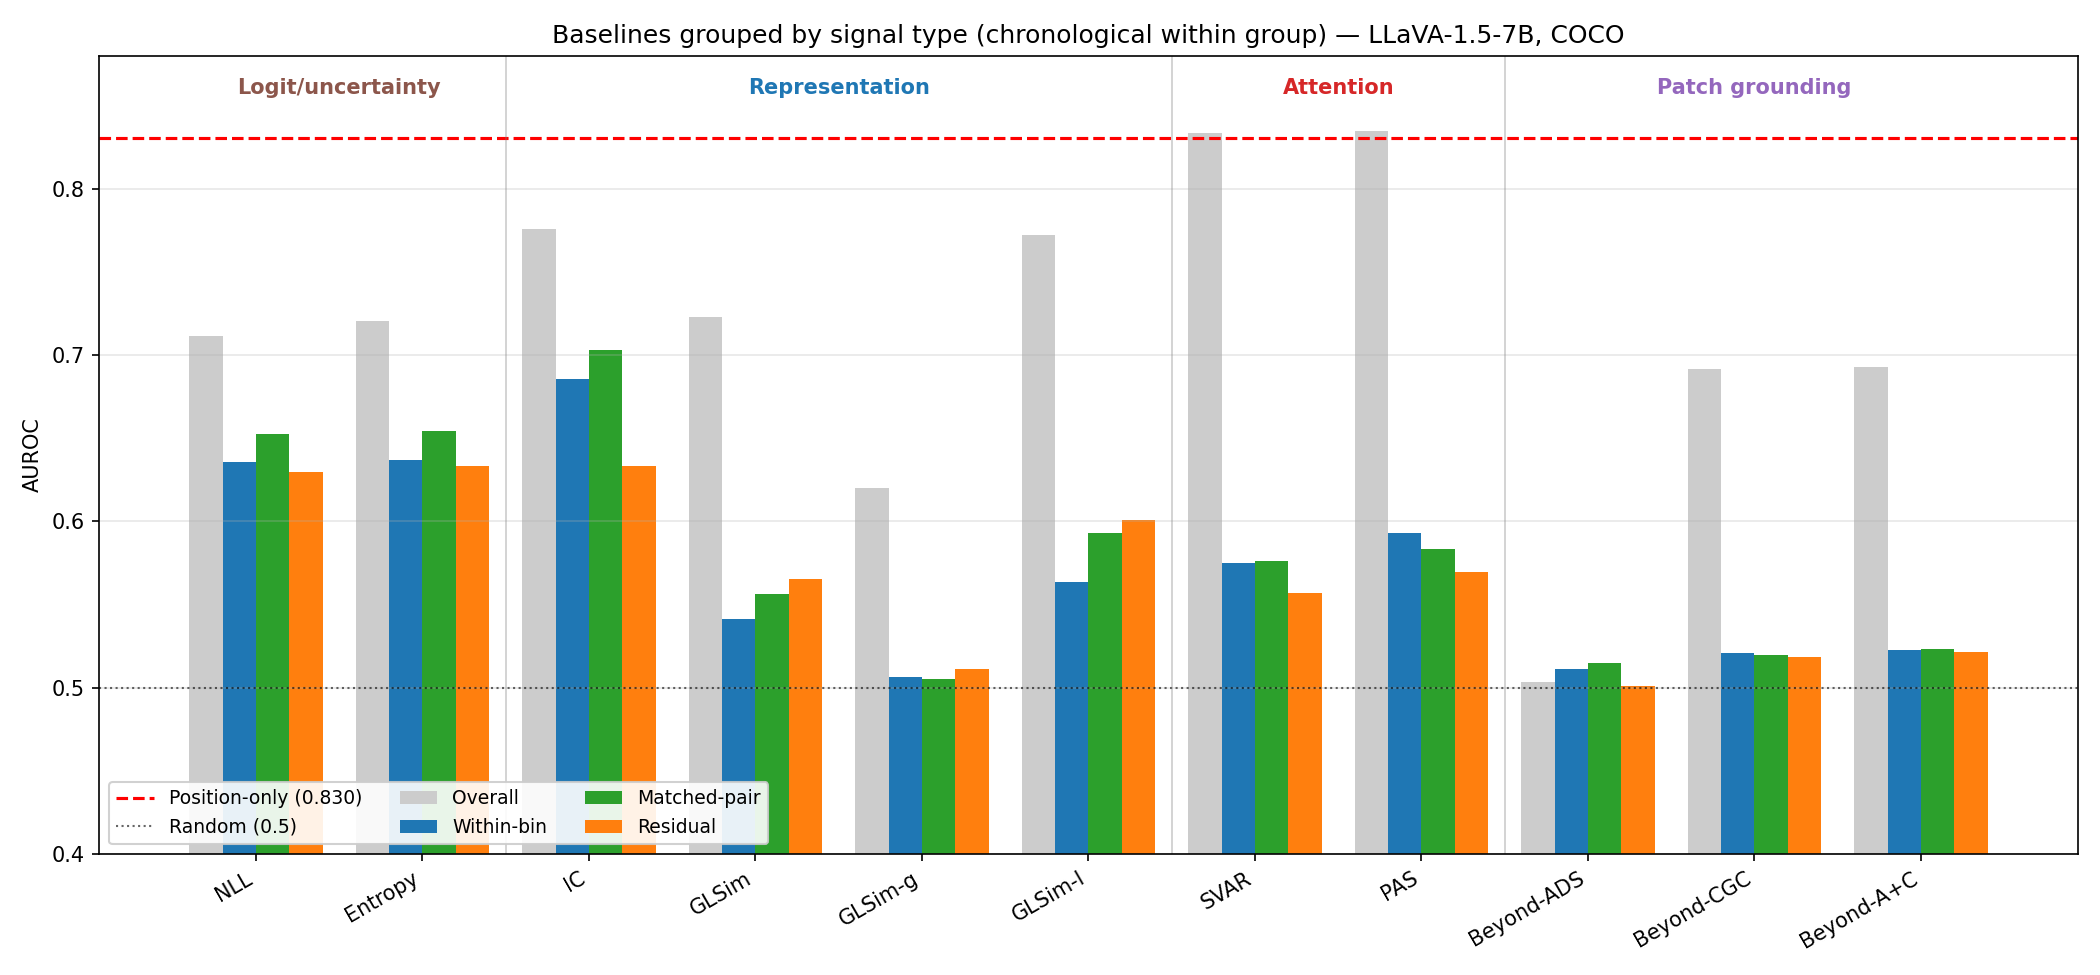
\includegraphics[width=0.95\textwidth]{assets/figures/fig_summary.png}
\caption{Overall vs.\ position-controlled AUROC by signal family. The dashed line marks position-only AUROC ($0.830$); the dotted line marks chance. PAS and SVAR look strongest in aggregate but collapse under position control.}
\label{fig:summary}
\end{figure*}

\begin{figure}[t]
\centering
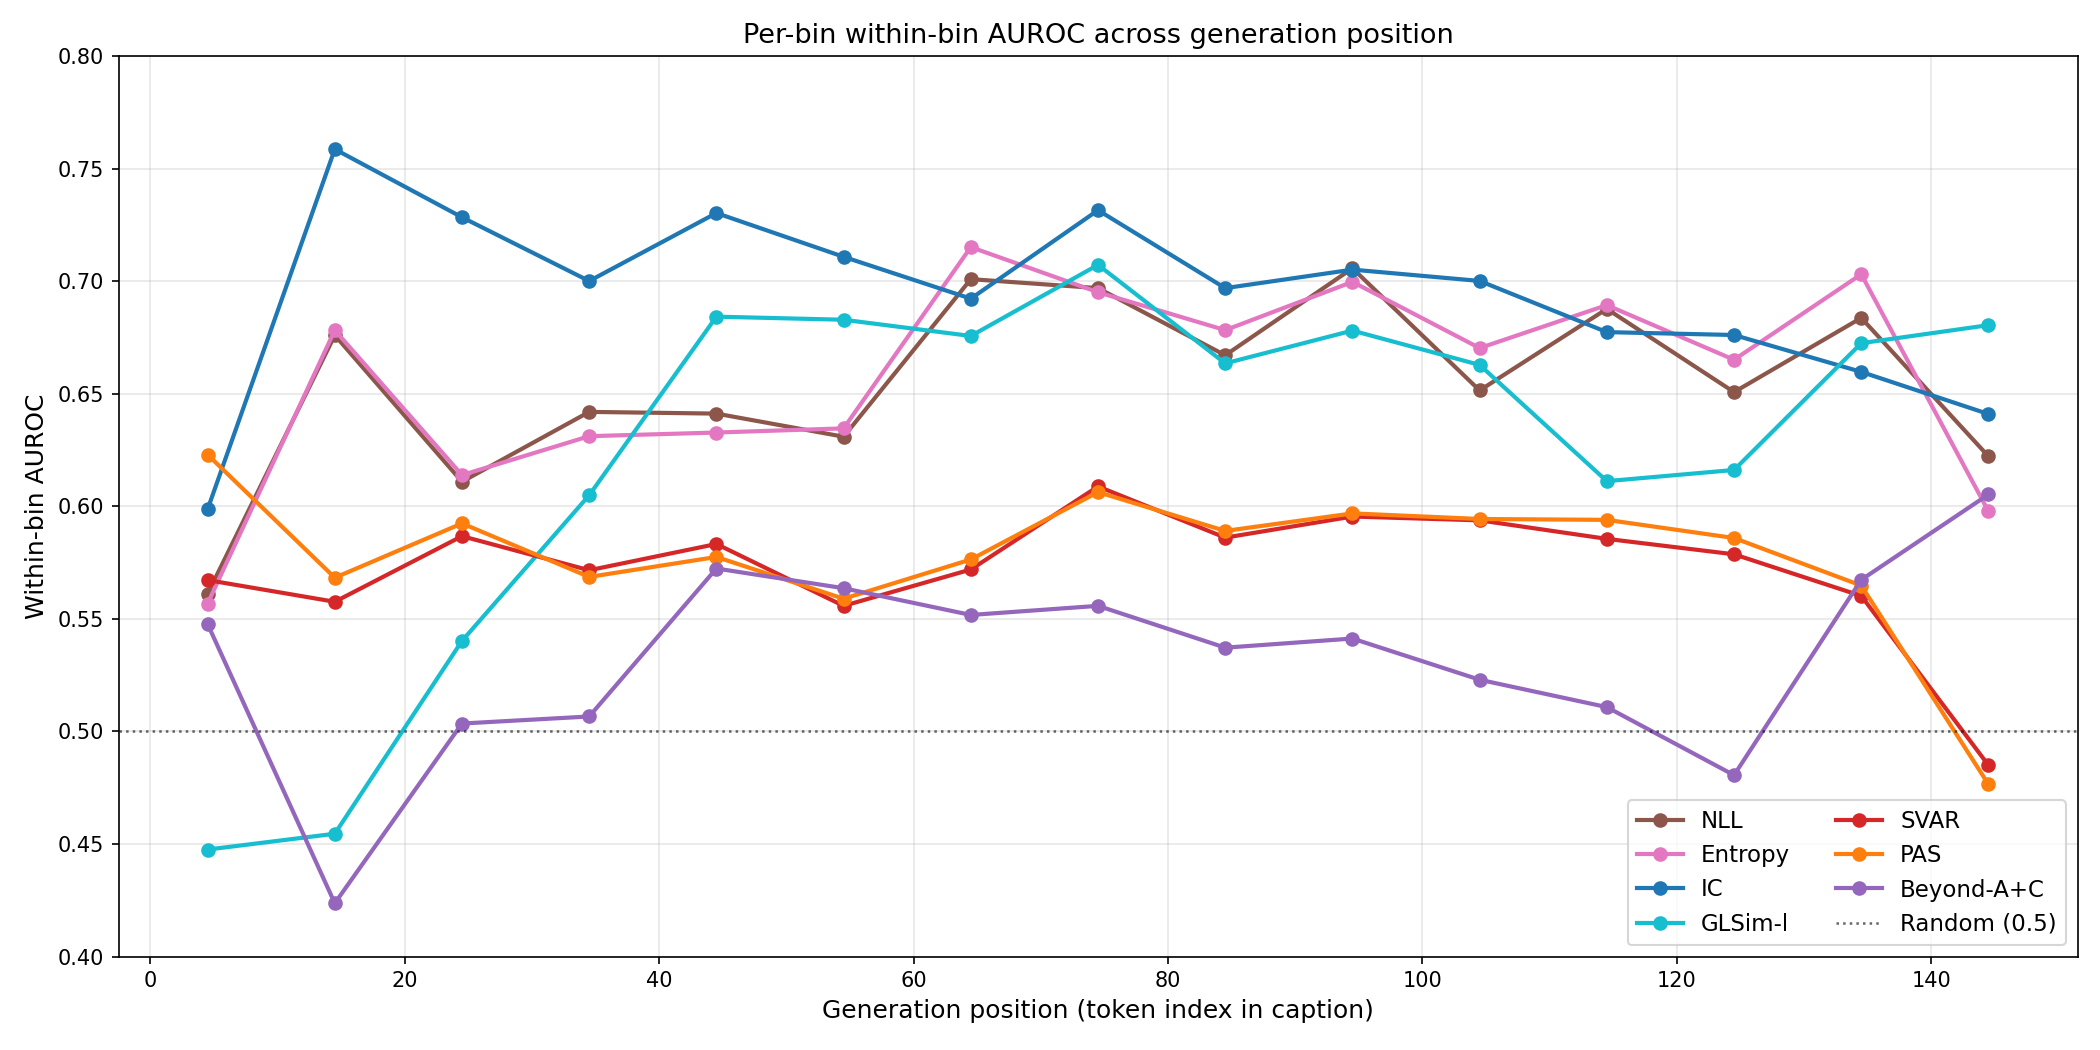
\includegraphics[width=\columnwidth]{assets/figures/fig_per_bin.png}
\caption{Within-bin AUROC across generation position. IC is consistently stronger than attention-mass scores; PAS/SVAR remain near $0.55$--$0.60$.}
\label{fig:perbin}
\end{figure}

\paragraph{A clean split between families.} Table~\ref{tab:main} and Figure~\ref{fig:summary} show that overall AUROC and position-controlled AUROC tell opposite stories for the attention family. PAS and SVAR have the two \emph{highest} overall AUROCs ($0.835$, $0.834$)---at or above the position-only floor---yet their within-bin AUROC is only $0.593$ and $0.575$. Expressed as retained above-chance signal, $(\text{within-bin}-0.5)/(\text{overall}-0.5)$, PAS keeps $28\%$ and SVAR $22\%$. By contrast, IC keeps $67\%$ ($0.686$ within-bin), entropy $62\%$, and NLL $64\%$. The fine-grained patch-grounding detectors (Beyond-*) are near chance on all position-controlled metrics. There is essentially no middle ground: methods retain either $\sim$$60$--$67\%$ or $\sim$$12$--$28\%$.

\paragraph{The split tracks signal source, not recency.} Ordering methods by proposal date (Figure~\ref{fig:summary}) shows the earliest representation method, IC, remains the strongest position-controlled detector, ahead of every later attention/grounding method. Improvements in overall AUROC over time largely reflect better fitting of the position prior, not new position-independent signal.

\paragraph{Per-position view.} Figure~\ref{fig:perbin} confirms the gap is consistent across positions: IC dominates in nearly every bin, whereas PAS/SVAR remain flat near $0.55$--$0.60$ throughout. The advantage of representation/uncertainty signals is not concentrated in a few easy bins.

\paragraph{What survives control is not simply ``more vision''.} The robust detectors are not the ones that most directly count image attention. Entropy and NLL read the output distribution, and IC reads whether internal visual representations support the object through a logit-lens style compatibility signal. These scores are imperfect, but they do not collapse as sharply when position is fixed. This suggests that the model contains object-relevant information, yet the information is not captured by coarse attention mass. In other words, the failure is not that LVLMs have no grounding signal; the failure is that attention mass is a poor stand-alone extractor of that signal.

\paragraph{The gap survives stronger matching.} Table~\ref{tab:strong-controls} reports the additional controls. The same-object-word matched AUROC is the most direct response to the possibility that detectors exploit object-frequency effects rather than grounding: IC, entropy, and NLL remain around $0.70$, while PAS and SVAR remain near $0.56$--$0.57$. Nonlinear residuals tell the same story. Cubic residual AUROC is $0.633$--$0.634$ for IC/entropy/NLL but only $0.558$ for PAS and $0.546$ for SVAR. Thus the detection split is not an artifact of the particular binning or residualization choice.

\begin{table}[t]
\centering
\scriptsize
\setlength{\tabcolsep}{3.0pt}
\begin{tabular}{lccc}
\toprule
Method & Same-word match & Cubic residual & Retained \\
\midrule
NLL & 0.698 & 0.630 & 0.93 \\
Entropy & 0.712 & 0.634 & 0.96 \\
IC & \textbf{0.716} & 0.633 & 0.78 \\
PAS & 0.569 & 0.558 & 0.21 \\
SVAR & 0.565 & 0.546 & 0.20 \\
GLSim-local & 0.615 & 0.600 & 0.42 \\
SinkDetect-global & 0.477 & 0.484 & -0.08 \\
SinkDetect-CLC & 0.592 & 0.550 & 0.64 \\
\bottomrule
\end{tabular}
\caption{Additional controls on saved per-object scores. Same-word match pairs hallucinated and grounded mentions of the same object word within $\pm5$ generated tokens. Retained is $(\mathrm{same\mbox{-}word}-0.5)/(\mathrm{overall}-0.5)$. Attention mass scores remain weak under object-category control.}
\label{tab:strong-controls}
\end{table}
 

\subsection{Stress Test: SinkDetect}
\label{sec:sinkdetect}

A natural objection is that attention \emph{shape}, as opposed to attention \emph{mass}, might carry position-independent grounding signal that prior attention detectors simply read too crudely. To test this directly we build SinkDetect, a detector designed to read shape.

\paragraph{Method.} Let $\tilde a_q$ be the object query's attention row restricted to the visual-token span, with detected sink columns removed and the remainder $L_1$-normalized to a distribution. SinkDetect scores $\tilde a_q$ along three axes. \emph{(i) Counterfactual visual grounding (CVG):} the negative divergence $-\mathrm{KL}(\tilde a_q \,\|\, \pi)$ and $-\mathrm{JSD}(\tilde a_q, \pi)$ from null distributions $\pi$ taken as the average instruction-token attention, a uniform distribution, and a local non-object null; closeness to a language-prior null is treated as evidence of hallucination. \emph{(ii) Concentration:} the entropy $H(\tilde a_q)$ and top-$k$ mass, testing whether attention is diffuse. \emph{(iii) Cross-layer consistency (CLC):} the generalized Jensen--Shannon divergence among the per-layer distributions, testing whether the attended region is stable across depth. Sinks are visual tokens with anomalously large pre-RoPE key norm that absorb attention mass without carrying semantics; removing them, together with an optional top-mass mask, forms a $2\times2$ purification ablation, each variant optionally recomputed on a no-RoPE branch. The full score set spans these axes $\times$ purification variants $\times$ per-layer/global aggregation. Crucially, because every distribution is $L_1$-normalized before scoring, total attention mass---the position-confounded quantity---is divided out by construction; SinkDetect therefore isolates \emph{shape}.

\paragraph{Result.} Despite this design, SinkDetect's best within-bin AUROC is $\approx$$0.50$, and its residual AUROC is $0.49$--$0.51$. Its highest \emph{overall} AUROC ($0.81$) again comes from a concentration score that correlates with position. Normalizing away mass does not help, because the confound also lives in the \emph{shape} of the normalized distribution: early tokens attend broadly (high entropy), late tokens attend narrowly, independent of grounding. We read this as evidence that the limitation is structural to attention-magnitude--derived signals on this model, not a failure of feature engineering: even purpose-built shape features, with sinks and dominant patches removed, recover no position-independent signal.

The SinkDetect result is useful precisely because it is a failed stress test. It removes the most obvious defects of attention-mass detectors: sink tokens, dominant visual patches, total mass, and RoPE-related ablations. Yet the best global score still comes from a feature whose distribution changes with decoding progress. This narrows the interpretation of the detection study. PAS and SVAR do not fail only because they use a crude scalar; a more careful hand-crafted attention shape also fails when forced to discriminate at comparable generation positions. A positive attention-based detector will likely need head-specific selection, learned verification, or external grounding constraints rather than another global average over visual rows.
 \section{Mitigation Findings}
\label{sec:mitigation}

The detection results raise a natural question: if attention scores are unreliable proxies for grounding, do attention interventions reliably reduce hallucination? We evaluate this directly by comparing vanilla generation with three training-free attention interventions. Each method is evaluated on identical POPE and CHAIR samples, and all deltas are computed relative to vanilla.
The reproduction scope is deliberately component-level: PAI denotes only its image-attention logit boost, excluding its CFG/contrastive branch; ClearSight denotes VAF mid-layer scaling; and VisAttnSink denotes sink redistribution. This scope keeps the test aligned with our question: whether attention manipulation itself verifies object presence.

\begin{table*}[t]
\centering
\small
\setlength{\tabcolsep}{4.2pt}
\begin{tabular}{lrrrrrrrr}
\toprule
Method & $\Delta$Acc & $\Delta$MCC & $\Delta$Yes & $\Delta$TPR & $\Delta$FPR & $\Delta C_i$ & $\Delta$Obj & $\Delta$Hall \\
\midrule
PAI-attn-only & -0.001 & -0.002 & -0.004 & -0.005 & -0.003 & +0.000 & +0.14 & +0.02 \\
ClearSight    & -0.001 & -0.006 & +0.036 & +0.035 & +0.038 & +0.001 & -0.11 & -0.01 \\
VisAttnSink   & -0.004 & -0.008 & +0.006 & +0.002 & +0.009 & +0.009 & +0.24 & +0.10 \\
\bottomrule
\end{tabular}
\caption{Mitigation behavior relative to vanilla. POPE deltas are macro-averaged over random/popular/adversarial splits; CHAIR deltas are over $5{,}000$ captions. ClearSight's recall gain is matched by FPR growth, while VisAttnSink increases hallucinated object mentions.}
\label{tab:pope-mitigation}
\end{table*}
 

\begin{table}[t]
\centering
\scriptsize
\setlength{\tabcolsep}{3.1pt}
\begin{tabular}{lrrrr}
\toprule
Method & $\Delta V$ & $\Delta$TPR & $\Delta$FPR & TP/FP $V$ \\
\midrule
PAI & +0.038 & +0.000 & +0.000 & .103/.105 \\
ClearSight & -0.017 & +0.017 & +0.033 & .063/.063 \\
VisSink & +0.002 & +0.017 & +0.017 & .067/.071 \\
\bottomrule
\end{tabular}
\caption{Adversarial POPE attention-shift audit ($120$ samples). $\Delta V$ is matched active-layer visual-mass change vs.\ vanilla; TP/FP $V$ reports post-intervention visual mass for true and false positives. Visual mass is not selective for correct object presence.}
\label{tab:attention-audit}
\end{table}
 

\paragraph{POPE gains can be answer-prior shifts.} Table~\ref{tab:pope-mitigation} shows that ClearSight is the only method with a positive macro F1 delta, but its gain follows the pattern of a yes-prior shift. It raises TPR by $3.5$ points and FPR by $3.8$ points, while MCC decreases. On adversarial POPE specifically, ClearSight increases TPR by $3.5$ points but FPR by $5.5$ points, causing accuracy to drop by one point. Thus the method makes the model more likely to answer ``yes,'' but does not improve object-presence discrimination. PAI-attention-only is nearly neutral but slightly worse, suggesting that PAI's full reported benefit may depend on its contrastive/CFG component rather than attention amplification alone. VisAttnSink mildly increases yes rate and FPR while reducing accuracy and MCC.

\paragraph{Captioning does not show hidden mitigation.} The CHAIR columns of Table~\ref{tab:pope-mitigation} rule out the possibility that POPE misses a captioning improvement. None of the interventions lowers CHAIR$_i$. PAI-attention-only and VisAttnSink make captions more object-rich; the latter increases hallucinated object mentions by $0.10$ per caption on average. ClearSight slightly shortens captions and mentions fewer objects, but still does not reduce CHAIR. These patterns support the same interpretation as the detection study: visual attention manipulation changes output behavior, but does not provide calibrated evidence verification for object claims.

\paragraph{Attention changes are real but not selective.} Table~\ref{tab:attention-audit} shows why the behavioral gains are misleading. PAI increases matched active-layer visual mass by $+0.038$ and reduces prefix/sink mass, yet every adversarial POPE decision is unchanged. Moreover, PAI false positives receive slightly \emph{higher} visual mass than true positives ($0.105$ vs.\ $0.103$). ClearSight raises TPR but raises FPR twice as much on the same subset, reducing MCC; its TP and FP visual masses are nearly identical. Visual Attention Sink moves attention in the intended direction only weakly ($+0.002$ visual mass, $-0.005$ sink mass) and increases TPR and FPR by the same amount. The interventions therefore change routing, but the routing change is not selective for object presence.

\paragraph{Why the interventions fail.} The three methods fail for related but distinct reasons. PAI-attention-only adds a positive offset proportional to the magnitude of image-attention logits, so it strengthens whatever image-attention pattern already exists; it does not test whether the attended patch supports the queried object. ClearSight applies a broader mid-layer amplification of text-to-image attention while suppressing prefix attention, which can make image evidence more influential but can also shift the model toward affirmative answers whenever the question mentions a plausible object. Visual Attention Sink redistributes mass from high-activation sink tokens to visual tokens, increasing visual-token participation during decoding, but this can make generation more object-rich rather than more faithful. In all three cases, the operation changes the routing of computation but never introduces an explicit object-presence verifier. This explains why POPE recall and false-positive rate move together, and why richer captions can contain more hallucinated objects.
 \section{Associated Evidence Audit}
\label{sec:associated-audit}

\noindent The detection and mitigation results point to the same missing criterion: target-discriminative evidence. A method can attend to the image, or even to a semantically meaningful region, without verifying the queried object. We therefore introduce an associated-evidence audit that separates three negative settings: random negatives, co-occurrence negatives, and semantic-neighbor negatives. In all three settings the target object is absent; the difference is whether the image contains an object or context that makes the target plausible.

\paragraph{Audit construction.}
For each target object $o$, we construct absent-object questions from COCO images where $o$ is not annotated. Random negatives are sampled without requiring related objects. Co-occurrence negatives require at least one object that frequently co-occurs with $o$ in the COCO training annotations. Semantic-neighbor negatives require an object whose name is close to $o$ under a text-embedding similarity matrix and passes a manual sanity filter. Typical pairs include sink--toilet, fork--knife, bus--truck, cup--bottle, and bed--couch. This construction targets the failure mode in which attention selects visually plausible associated evidence rather than target evidence.

\paragraph{Evaluation.}
For detection, we report each score's false-grounded rate on the negative slices at a fixed threshold calibrated on the full validation set, together with the score gap between target-present positives and semantic-neighbor negatives. For mitigation, we report yes rate, FPR, and $\Delta\mathrm{TPR}-\Delta\mathrm{FPR}$ separately on the three negative slices. For attention audits, we compare the intervention-induced visual-attention change on true positives and semantic-neighbor false positives. A method passes the audit only if its signal or intervention remains selective for target presence rather than merely increasing evidence plausibility.

\TODO{Run the semantic-neighbor audit. Required outputs: detection false-grounded rate by negative type, mitigation yes/FPR by negative type, TP vs semantic-neighbor-FP attention mass, and 3--5 qualitative cases with real images and attention maps.}
 \section{Discussion}
\label{sec:discussion}

\noindent Our results should not be read as evidence that attention is irrelevant to grounding. IC, uncertainty baselines, and preliminary per-head probes all suggest that LVLMs contain object-relevant information, and some of that information may be attention-derived. The negative result is narrower and more actionable: raw attention mass, mean-over-head attention shape, and unselective attention amplification are not reliable certificates of grounding.

\noindent The practical implication is that attention-based claims need selectivity controls. A detector should show that its score separates present from absent objects at comparable generation positions and object categories. A mitigation method should show that its routing change improves true positives more than false positives, rather than merely increasing yes rate or caption object richness. Semantic-neighbor negatives make this requirement concrete by testing the cases where associated evidence is present but target evidence is absent.

\noindent This framing leaves room for better attention methods. Head selection, learned verification heads, detector-assisted grounding, and counterfactual region tests may pass the proposed controls. The contribution of this paper is to make those controls necessary before attention-based gains are interpreted as hallucination detection or mitigation.
 \section{Conclusion}

This paper re-evaluates attention-based hallucination methods through the lens of evidence verification. For detection, we show that generation position can explain much of the apparent success of attention-based scores, and that position-controlled evaluation sharply separates attention-mass scores from representation and uncertainty baselines. For mitigation, we show that attention interventions can alter output behavior without reliably reducing hallucinations: ClearSight shifts POPE answers toward ``yes,'' PAI-attention-only changes attention without changing decisions, and Visual Attention Sink increases hallucinated object mentions in captions.

The central lesson is simple but important: attention may reveal where a model looks, but it does not by itself establish whether the model verifies what it says. The critical distinction is target-discriminative evidence. A model can attend to a real, semantically associated region and still make a false object claim; amplifying that attention can strengthen plausibility rather than verification. Future hallucination methods should treat attention as a candidate feature to be controlled, selected, or learned from, not as a direct certificate of grounding. A detector or mitigation method should earn its claim by showing that its signal remains selective under position, category, answer-prior, and semantic-neighbor controls.
 \section*{Limitations}

Our empirical scope is intentionally narrow but diagnostic: one backbone, COCO-derived object hallucination labels, and attention-intervention components rather than every full mitigation pipeline. This scope is enough to establish the proxy failure in the tested setting, but not enough to claim that all attention-based methods fail. The position confound is correlational, although strong; prompt-level or decoding-level interventions on generation position would further strengthen the evidence. Several baselines are ports or reimplementations, so official-code parity checks remain important for final submission. Head-selection mitigation, learned verification heads, and detector-assisted grounding may pass the controls proposed here. The point of this paper is to make those controls necessary before attention-based gains are interpreted as hallucination mitigation.
 
\appendix
\section{Per-bin AUROC table}
\label{sec:appendix}
A full per-bin breakdown (AUROC for every method in every position bin) accompanies the released code and reproduces Figure~\ref{fig:perbin}.
 
\bibliography{custom}

\end{document}
